% Канонический TikZ-рисунок варианта 18. Править только здесь.
\long\def\figStereoV18{%
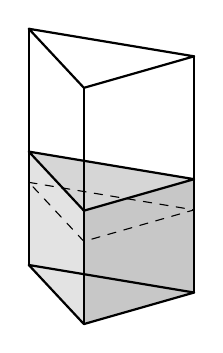
\begin{tikzpicture}[
  scale=1,
  line cap=round,
  line join=round
]
  % Верхнее основание призмы
  \coordinate (A) at (-0.9,2.7);
  \coordinate (B) at (1.2,2.35);
  \coordinate (C) at (-0.2,1.95);

  % Нижнее основание призмы
  \coordinate (A1) at (-0.9,-0.3);
  \coordinate (B1) at (1.2,-0.65);
  \coordinate (C1) at (-0.2,-1.05);

  % Новый уровень жидкости — 29 см
  \coordinate (A29) at (-0.9,1.14);
  \coordinate (B29) at (1.2,0.79);
  \coordinate (C29) at (-0.2,0.39);

  % Первоначальный уровень жидкости — 25 см
  \coordinate (A25) at (-0.9,0.75);
  \coordinate (B25) at (1.2,0.40);
  \coordinate (C25) at (-0.2,0);

  % Жидкость после погружения детали
  \fill[black!16]
    (A1) -- (B1) -- (B29) -- (A29) -- cycle;

  \fill[black!22]
    (B1) -- (C1) -- (C29) -- (B29) -- cycle;

  \fill[black!11]
    (C1) -- (A1) -- (A29) -- (C29) -- cycle;





  % Рёбра призмы
  \draw[thick]
    (A) -- (B) -- (C) -- cycle;

  \draw[thick] (A) -- (A1);
  \draw[thick] (B) -- (B1);
  \draw[thick] (C) -- (C1);

  \draw[thick]
    (A1) -- (B1) -- (C1) -- cycle;

  % Уровень до погружения детали
  \draw[dashed]
    (A25) -- (B25) -- (C25) -- cycle;

  % Уровень после погружения детали
  \draw[thick]
    (A29) -- (B29) -- (C29) -- cycle;
\end{tikzpicture}
}
